\chapter{Methodology}
\label{chapter2}

\section{Methodology Overview}

This chapter defines the methodological design used to develop and evaluate the lightweight prediction scheduling pipeline used in this edge Kubernetes study. It specifies the system design, study environment, data-governance rules, predictor-selection path, policy locking procedure, and evaluation protocol used for the final scheduler claim. The replication studies that justify anomaly-source selection are documented separately in Appendix~\ref{appendixB}.

\subsection{System Design}

The system is a custom scheduler built from two decision signals. The first is a short-horizon resource predictor that estimates future node load from recent telemetry windows. The second, retained on the basis of the replication evidence in Appendix~\ref{appendixB}, is a runtime NSA-based anomaly monitor that estimates whether a node is behaving abnormally from recent telemetry history. At decision time these signals are combined with workload size, capacity, contention, and safety terms to produce a ranked list of feasible nodes.

Figure~\ref{fig:system-design} summarises this conceptual design and shows how telemetry-derived prediction and anomaly signals are combined within the custom scheduler at decision time.

\begin{figure}[htbp]
    \centering
    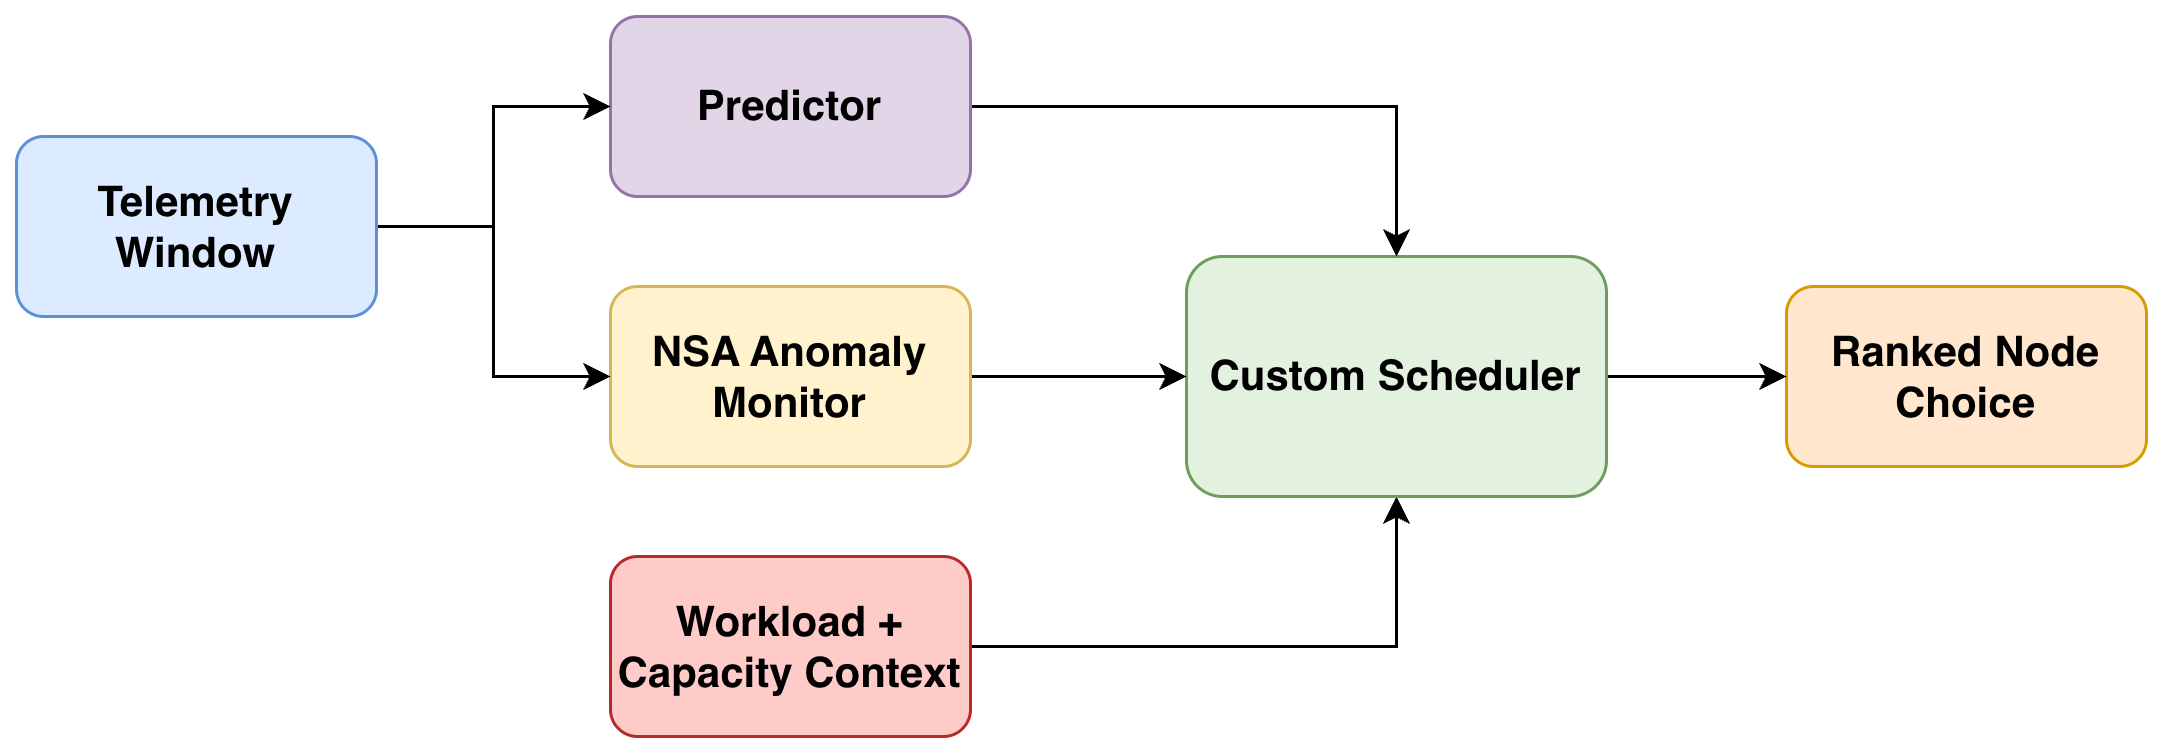
\includegraphics[width=0.95\textwidth]{./system-design.png}
    \caption{Conceptual system design of the scheduler combining anomaly monitoring and prediction.}
    \label{fig:system-design}
\end{figure}

\subsection{Research Questions and Hypotheses}

The methodology addresses the following research questions, which motivate the end-to-end pipeline:

\begin{itemize}
\item \textbf{RQ1:} Can a custom scheduler that combines anomaly monitoring and prediction improve placement quality compared to the default Kubernetes scheduler in an edge cluster?
\item \textbf{RQ2:} Can those improvements be achieved while preserving low scheduling overhead suitable for edge settings?
\item \textbf{RQ3:} Does the locked hybrid policy family transfer from offline replay audit to online deployment against the default scheduler?
\end{itemize}

These questions are operationalised through the following hypotheses:

\begin{itemize}
\item \textbf{H1:} The custom scheduler improves safe placement rate and reduces anomalous or highly contended placement compared to the default Kubernetes scheduler.
\item \textbf{H2:} The custom scheduler does not introduce practically significant scheduling latency or pod startup time overhead.
\item \textbf{H3:} The locked hybrid policy family yields positive utility delta when deployed online against the default scheduler across repeated matched-arm trials.
\end{itemize}

\textbf{Exploratory question:} In a supplementary Pi-inclusive extension, can the locked custom arm be exposed to a heterogeneous worker pool through workload-specific eligibility without collapsing into blanket Pi usage or blanket Pi avoidance?

\subsection{End-to-End Pipeline}

The methodological pipeline is organised into two linked stages.

\textbf{Offline development}
\begin{enumerate}
\item \textbf{Telemetry collection and preprocessing.} A governed telemetry corpus is collected from the live K3s cluster, cleaned, labelled, and filtered to preserve only runs with the required artifacts and worker coverage.
\item \textbf{Predictor training and validation.} Per-node lightweight regressors are trained on the governed development slice using leakage-safe scaling, phase-aware weighting, and post-fit calibration; their adequacy is checked on a strict holdout split before any live claim is made.
\item \textbf{Locked policy selection.} Internal prediction-only, anomaly-only, and hybrid policies are compared under replay audit, and a single safety-priority hybrid configuration is frozen before online deployment.
\end{enumerate}

\textbf{Online evaluation}
\begin{enumerate}
\setcounter{enumi}{3}
\item \textbf{Matched-arm execution and analysis.} Baseline and custom arms are executed on the live cluster, per-decision artifacts are retained, and the final summary is generated from the resulting scheduling traces.
\end{enumerate}

\section{Cluster and Data Pipeline}

\subsection{Cluster Environment}

The study environment comprised a K3s control plane, a homogeneous cloud worker pool, and a supplementary heterogeneous worker. This full topology supported telemetry collection, predictor coverage, and the supplementary Pi-inclusive extension. Hardware specifications are summarised later in Chapter~\ref{chapter3}, Table~\ref{tab:ch3-cluster-nodes}.


K3s was used as the Kubernetes distribution in place of the full upstream package. As described in Chapter~\ref{chapter1}, K3s is designed specifically for resource-constrained and remote environments, which makes it a closer approximation of realistic edge cluster hardware than a standard Kubernetes installation on cloud VMs.

Netdata was selected as the telemetry platform because it is built for edge-first deployment: it delivers per-second metric precision, maintains a minimal CPU and memory footprint during collection, and operates autonomously when upstream connectivity is interrupted.

Operational access relied on Google Cloud SSH for the cloud VMs and Tailscale as the private remote-access layer spanning the cloud nodes, the heterogeneous worker, and the local operator environment. This infrastructure enabled experiment execution and telemetry retrieval, but it was not part of the scheduler decision signal itself.

\subsection{Data Collection, Labelling and Governance}

Only metric streams exposed consistently across the cluster were admitted into the governed corpus. Table~\ref{tab:ch2-telemetry-surface} summarises the collected metric surface and distinguishes between the features retained by the final predictor and ranker and those kept only for diagnostic context.

\begin{table}[h]
\centering
\small
\begin{adjustbox}{max width=\textwidth}
\begin{tabular}{llll}
\hline
\textbf{Netdata chart} & \textbf{Derived metric(s)} & \textbf{Retained live?} & \textbf{Role} \\
\hline
\texttt{system.cpu} & \texttt{cpu\_user}, \texttt{cpu\_system}, \texttt{cpu\_iowait} & user/system only & Compute pressure; \texttt{iowait} kept for diagnostics \\
\texttt{system.ram} & \texttt{ram\_used} & yes & Memory saturation risk \\
\texttt{system.net} & \texttt{net\_received}, \texttt{net\_sent} & yes & Traffic-driven load \\
\texttt{system.load} & \texttt{load1} & no & Diagnostic context only \\
\hline
\end{tabular}
\end{adjustbox}
\caption{Telemetry surface used in the governed corpus and final scheduler pipeline.}
\label{tab:ch2-telemetry-surface}
\end{table}

These metrics were chosen because they cover the resource subsystems the scheduler must discriminate at decision time. CPU user and system activity represent short-horizon compute pressure, RAM usage reflects memory saturation risk, and network ingress and egress capture traffic-driven load that would be hidden by a CPU-only view. Timing outcomes such as scheduling latency and startup time are evaluated separately from Kubernetes traces rather than inferred from telemetry alone.

Sampling was fixed at one second because both the online warm-up and anomaly-history buffers operate over short windows, and the stress interventions evolve on the order of seconds. A coarser polling rate would smooth transient contention changes that the live ranker is designed to react to, while a substantially faster rate would increase collection cost without changing the practical decision horizon.

Phase structure imposes controlled operating contexts on the telemetry corpus. Normal phases provide low-interference baselines, targeted stress phases create labelled anomalous intervals, and recovery periods show how quickly nodes return toward baseline behaviour. In the scheduler protocol the same phase structure creates comparable decision contexts across arms, allowing later analysis to distinguish behaviour under CPU, memory, and mixed interference.

Labelling is phase-aware and node-aware: during a stress phase, only the targeted node is labelled anomalous. This preserves causal alignment between injected stress and anomaly labels. Control-node telemetry is collected for full-cluster observability, but worker-only filtering is applied for scheduler-oriented evaluation because workload placement decisions are made on worker nodes.

The governed corpus follows three rules:

\begin{itemize}
\item \textbf{Split locking.} Strict holdout runs are fixed in split configuration and excluded from development-stage replay audit.
\item \textbf{Inclusion criteria.} Runs missing required artifacts are excluded from model and evaluation input.
\item \textbf{Operational repair policy.} Interrupted collections are resumed from a specified run index; invalid partial runs are removed before retry.
\end{itemize}

\subsection{Feature Engineering and Preprocessing Choices}

The predictor and live ranker consume the chosen per-node features \texttt{cpu\_user}, \texttt{cpu\_system}, \texttt{ram\_used}, \texttt{net\_received}, and \texttt{net\_sent}. For the replication appendix (Appendix~\ref{appendixB}), these are also aggregated into CPU and NET composites where required by the detector studies.

Preprocessing differs by stage:

\begin{itemize}
\item \textbf{Anomaly stage.} Rolling-mean smoothing and min-max normalisation are used to study detector separability under realistic edge noise.
\item \textbf{Prediction stage.} Leakage-safe scaling is applied by fitting the scaler on the training period only and then transforming the full sequence for window construction.
\item \textbf{Online evaluation stage.} Recent telemetry snapshots are ranked directly from Netdata-derived features, while workload requests and exported node capacities are injected only at decision time as execution context rather than as learned time-series features.
\end{itemize}

This separation keeps detector replication, predictor fitting, and online evaluation focused on different methodological questions while preserving a compatible telemetry surface across stages.

\section{Predictive Modelling Method}

\subsection{Predictor Design and Training Protocol}
\label{sec:predictor-design}

The predictor is a lightweight sliding-window regression model trained per worker node. The candidate model family comprised linear and ridge regression, with model selection on the governed development slice retaining the linear variant for the final locked pipeline.

Given input sequence \(x_t\), training windows are formed as:

\[
X_i = [x_i, x_{i+1}, \dots, x_{i+w-1}], \quad y_i = x_{i+w+h-1}
\]

where each \(x_t\) contains the five telemetry features. Training uses:

\begin{itemize}
\item \textbf{Leakage-safe split:} temporal split before scaling, with scaler fit on the training period only.
\item \textbf{Phase-aware weighting:} CPU and mixed stress targets receive higher sample weights because scheduling decisions during stressed operation are more important than during quiescent operation.
\item \textbf{Post-fit calibration:} per-feature linear correction \(\hat{y}' = a\hat{y} + b\) learned on a calibration tail of the training data.
\end{itemize}

This model family was selected to preserve low inference cost while retaining sufficient short-horizon expressiveness for scheduler ranking. Rolling-origin cross-validation on the development corpus identified the \((w{=}5, h{=}3)\) configuration as the best RMSE trade-off, and strict holdout confirmation retained that RMSE-led ordering against naive baselines.


\subsection{Predictor Evaluation Method}

Predictor quality is evaluated independently of scheduler outcomes using MAE, RMSE, and sMAPE:

\begin{itemize}
\item \textbf{MAE:} direct average magnitude error.
\item \textbf{RMSE:} error magnitude with stronger penalty on larger misses.
\item \textbf{sMAPE:} scale-aware relative error for bounded normalised series.
\end{itemize}

This stage validates forecasting adequacy only. Scheduler claims are made from replay and online placement metrics rather than from predictor error alone.


\section{Hybrid Scheduler Method}

\subsection{Node Risk and Scoring Formulation}

At each decision step, each candidate node receives three signals:

\begin{itemize}
\item \textbf{Base predicted load} from the node predictor.
\item \textbf{Anomaly risk} from a lightweight detector monitor.
\item \textbf{Workload capacity penalty} derived from the pod request and the node's allocatable CPU and memory.
\end{itemize}

If the predictor is not yet ready, or if a node lacks trained predictor artifacts, a bounded fallback load estimate is formed from current CPU, RAM, and network observations. This ensures the live ranker continues to operate on the selected worker set even when model coverage is incomplete.

For node \(i\), let \(\hat{L}_i\) denote base predicted load, \(R_i\) anomaly risk, \(C_i\) the workload capacity penalty, and \(\rho_i\) the observed relative CPU load at decision time. The live score is:

\[
\text{score}_i = w_p^{(i)}\,(\hat{L}_i + C_i) + \left(1-w_p^{(i)}\right)R_i + P_i^{\text{cont}} + P_i^{\text{safe}}
\]

where \(w_p^{(i)}\) is either a fixed prediction weight or an adaptively shifted value based on anomaly risk. The capacity term is defined as:

\[
C_i = \gamma\,\max\!\left(\frac{\text{cpu}_{\text{req}}}{\text{cpu}_{\text{cap},i}},\;\frac{\text{mem}_{\text{req}}}{\text{mem}_{\text{cap},i}}\right)
\]

with \(\gamma\) fixed before the live experiment. Explicit contention and safety penalties are then applied from the observed relative CPU level:

\[
P_i^{\text{cont}} = \lambda_c\,\max(0, \rho_i - \tau_c), \qquad
P_i^{\text{safe}} = \lambda_s\,\max(0, \rho_i - \tau_s)
\]

where \(\tau_c\) and \(\tau_s\) are the locked contention and safety thresholds, and \(\lambda_c\) and \(\lambda_s\) are the corresponding penalty factors. Lower total score indicates the preferred placement. When at least one node remains below the safety threshold, nodes above that threshold are additionally deprioritised through unsafe-node avoidance.

The NSA monitor remains one-class and history-based: each node's recent trajectory defines \textit{self} behaviour, while sampled detectors in non-self regions produce anomaly risk from nearest-detector distance. This preserves continuity with the replication evidence in Appendix~\ref{appendixB}, while the capacity and observed-load terms extend the ranker to live workload placement.


\subsection{Policy Variants and Comparison Surface}

Offline replay compares three internal policies on identical decision points:

\begin{itemize}
\item \textbf{Prediction-only:} \(w_p=1.0\), anomaly weight \(=0.0\).
\item \textbf{Anomaly-only:} \(w_p=0.0\), anomaly weight \(=1.0\).
\item \textbf{Hybrid:} prediction-led scoring with anomaly correction, workload capacity pressure, and explicit observed-load safety penalties.
\end{itemize}

The authoritative online evaluation uses a different comparison surface:

\begin{itemize}
\item \textbf{Default arm:} pods are left to the unmodified Kubernetes \texttt{default-scheduler}.
\item \textbf{Custom arm:} a live ranker selects the best node from telemetry, workload, and capacity context, after which the pod is bound authoritatively via \texttt{spec.nodeName}.
\end{itemize}

The remainder of this chapter uses \emph{offline replay} for the internal policy comparison and \emph{online matched-arm evaluation} for the external comparison against Kubernetes.


\section{Evaluation Protocol}

\subsection{Offline Policy Locking and Replay Audit}
\label{sec:offline-selection}

Policy locking separates configuration selection from final claim generation. During offline replay, prediction-only, anomaly-only, and hybrid candidates are compared on identical replay decision points over the governed development slice. Once that comparison identifies a single safety-priority family, its anomaly source, base weights, adaptive weighting rules, warm-up length, anomaly history settings, and safety penalties are frozen before any online run.

In this study the retained family remains prediction-led, keeps NSA as the anomaly source, and carries unchanged into the live comparison. Chapter~\ref{chapter3} reports the concrete locked configuration and the implementation artifacts that enforce it.

The replay objective is the protocol-defined utility:

\[
U = 0.45\,\text{safe} - 0.25\,\text{anom} - 0.15\,\text{contention} - 0.10\,\text{latency} + 0.05\,\text{fairness}
\]


\subsection{Online Matched-Arm Experiment (Stage-B)}

The authoritative comparison between the custom scheduler and the default Kubernetes scheduler is conducted as an online matched-arm experiment on the live K3s cluster. This experiment focuses on the primary research questions (RQ1-3) and is restricted to the homogeneous worker subset. This keeps both arms on the same feasible worker pool and makes the default scheduler baseline easier to interpret \cite{liu2024dynamic}.

\subsubsection{Experimental Design}

Each trial contains a normal phase and three stress phases (CPU, memory, and mixed). For each workload within each phase, arm order is counterbalanced so that odd-numbered trials execute baseline then custom, while even-numbered trials execute custom then baseline.

The two arms are:

\begin{enumerate}
\item \textbf{Baseline arm.} The workload manifest is submitted with worker pool eligibility constraints but without a forced node, leaving the placement decision to the unmodified \texttt{default-scheduler}.
\item \textbf{Custom arm.} The locked ranking policy evaluates the same eligible worker set immediately before submission and writes the selected node into \texttt{spec.nodeName}, making the placement decision authoritative.
\end{enumerate}

Stress profiles are rotated across the worker set to avoid coupling any single resource profile to a single node, and a short washout period is inserted after each decision to improve independence between successive placements.

\subsubsection{Workloads}

Phases are used as controlled operating contexts rather than as a simple ordering device. Each trial begins with a normal phase and then proceeds through CPU, memory, and mixed stress phases so that the same schedulers are evaluated under distinct forms of interference.

The workload set is intentionally small but differentiated. The \texttt{cpu-pod} emphasises compute demand, the \texttt{memory-pod} emphasises RAM pressure, and the \texttt{mixed-pod} combines both request types. Together they test whether scheduler choices remain coherent when workload demand either aligns with, or conflicts with, the currently stressed resource profile on a candidate node.

\subsubsection{Supplementary Pi-Inclusive  (Stage-C)}

This supplementary experiment addresses the exploratory heterogeneity question introduced earlier in the chapter. It does not replace the homogeneous worker claim; instead, it tests whether the locked custom arm can be exposed to a mixed-capacity worker pool through workload-specific eligibility without collapsing into blanket Raspberry Pi usage or blanket Raspberry Pi avoidance.

Only the eligibility surface changes. Lightweight workload variants make the Raspberry Pi a genuinely feasible target, while the ranking logic itself remains locked. The resulting analysis is therefore interpreted as a limitation study about heterogeneous transfer, not as replacement evidence for the authoritative homogeneous worker comparison.

\subsubsection{Metrics Collection}

Metrics are collected at two levels. Telemetry snapshots provide the node-state evidence used by the custom ranker, while Kubernetes scheduling traces provide the outcome evidence used to evaluate latency, placement, safety, and fairness. Keeping these layers separate ensures that the final evaluation focuses on deployment outcomes rather than on telemetry acquisition itself.

Within the final online summaries, a placement is marked high-contention when the chosen node's relative CPU reaches 1.1 and anomalous when it reaches 1.25; safe placement is the complement of that anomaly proxy. Placement fairness is reported as Jain's fairness over node placement counts \cite{jain1984quantitative}, capacity alignment measures how closely realised placement shares match the average of each node's CPU-share and memory-share capacity, stress-target avoidance is the percentage of decisions not placed on the actively stressed node, and expected-node match is the percentage of authoritative custom-arm decisions whose realised node matches the ranker's selected node.

\section{Software Management and Version Control}

The project was managed using Git with a remote repository hosted on GitHub. Development was organised across three major subsystems: \texttt{offline-replication} for anomaly-detection replication, \texttt{online-telemetry} for live cluster data collection, and \texttt{scheduler-prediction} for prediction, hybrid scoring, offline audit, and online evaluation.

The repository follows a modular directory structure:

\begin{itemize}
\item \texttt{anomaly-detection/offline-replication/} --- synthetic data generation, preprocessing, detection, and evaluation for the offline anomaly study.
\item \texttt{anomaly-detection/online-telemetry/} --- telemetry collection, preprocessing, and live-cluster detection experiments.
\item \texttt{scheduler-prediction/prediction/} --- predictor training, calibration, and validation.
\item \texttt{scheduler-prediction/custom-scheduler/} --- hybrid scheduler, offline replay audit, and live ranking engine.
\item \texttt{scheduler-prediction/baseline/} --- workload manifests and metric-collection helpers for scheduler comparison.
\item \texttt{scheduler-prediction/online/} --- authoritative matched-arm runner, analysis scripts, cluster configuration, and result artifacts.
\end{itemize}

Configuration files, evaluation protocols, environment templates, and saved model directories are version-controlled alongside the code they configure. This preserves reproducibility without relying on external documentation.

